\documentclass[tikz,border=2pt]{standalone}
\usepackage{amsmath,amssymb}
\usetikzlibrary{calc,arrows.meta}
\begin{document}
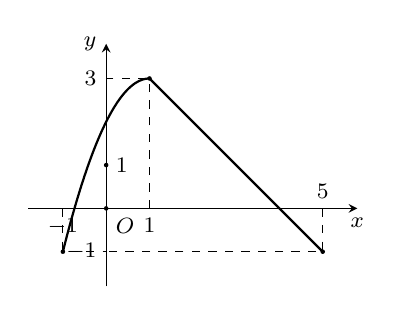
\begin{tikzpicture}[scale=0.55, font=\footnotesize, >=stealth]
	\draw[->] (-1.8,0) -- (5.8,0) node[below] {$x$};
	\draw[->] (0,-1.8) -- (0,3.8) node[left] {$y$};
	\fill (0,0) circle (1.5pt) node[below right] {$O$};
	\draw[dashed] (-1,0) node[below] {$-1$} -- (-1,-1) -- (0,-1) node[left] {$-1$};
	\draw[dashed] (1,0) node[below] {$1$} -- (1,3) -- (0,3) node[left] {$3$};
	\draw[dashed] (5,0) node[above] {$5$} -- (5,-1) -- (0,-1);
	\draw[thick, smooth, domain=-1:1] plot (\x, {-(\x-1)*(\x-1) + 3});
	\draw[thick, smooth, domain=1:5] plot (\x, {-(\x-1) + 3});
	\fill (-1,-1) circle (1.5pt) (1,3) circle (1.5pt) (5,-1) circle (1.5pt) (0,1) circle (1.5pt);
	\node[right] at (0,1) {$1$};
\end{tikzpicture}
\end{document}
